\documentclass{article}
\author{
    Epidemiological Modelling Unit,
    \\ School of Public Health and Preventive Medicine,
    \\ Monash University
}
\usepackage{graphicx}
\usepackage{biblatex}
\usepackage{threeparttable}
\usepackage{tabularx}
\usepackage[left=2.5cm,right=2.5cm]{geometry}
\bibliography{../../references/emu_library}

\title{Modelling methods, Bhutan application}

\begin{document}

\maketitle

% This file describes the general structure of some of our tb_dynamics models.

\section{Model Structure}

\subsection{General features}

We use a deterministic compartmental model including six types of compartments that represent 
different states of infection and disease. The model uses the same conceptual approach and similar 
assumptions to previously published models \cite{trauer-2017, ragonnet-2019, ragonnet-2021, ragonnet-2022}. 
Here we describe the model structure without treatment compartment and related factors. 
\newline
A susceptible compartment (S) is used to represent individuals who have 
never been infected with \emph{Mycobacterium tuberculosis (M.tb)}. Latent TB infection (LTBI) is modelled 
using two successive compartments: early latent (E) and late latent (L) to capture the declining risk of 
disease progression over time from infection \cite{ragonnet-2017}. The active disease compartment (I) represents 
individuals who have progressed to the active stage of TB disease. Diseased individuals who recover 
through self-cure progress directly to the recovered compartment (R).
\newline
Non-TB-related mortality is modelled by applying death rates to all model compartments. In addition, 
disease-specific mortality is implemented by applying increased mortality rates to the active disease 
compartments (I).
\newline
Reinfection occurs in the model in two different ways. First, latently infected individuals may be 
reinfected, with this process modelled using a flow from the late latent (L) to the early latent 
compartment (E). Second, individuals who have recovered from TB disease may be reinfected and 
return to the early latent compartment. The structure of our model allows for differential risk of 
infection for the currently and previously infected individuals, compared to the infection-naive 
individuals.
\begin{figure}[!htp]
    \vspace*{-1cm}
    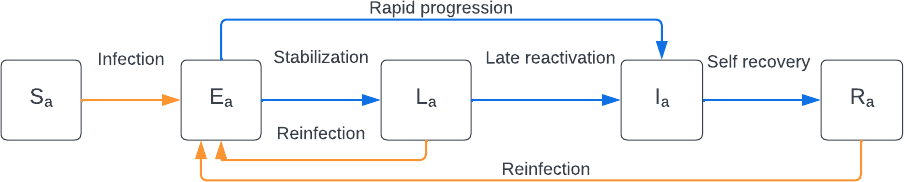
\includegraphics[width=\textwidth,height=\textheight,keepaspectratio]{images/model.png}
    \caption{Illustration of the model structure. 
    Boxes represent the different compartments types: susceptible (S), early latent (E), late latent (L), infectious (I), and recovered (R).
    The subscript indicates that compartments are stratified by age (a).}
    \label{fig:model}
\end{figure}

\subsection{Stratification by age}
The model is stratified using five categories: 0-4, 5-14, 15-34, 35-49 and 50+ years old. We assume 
heterogeneous mixing by age using an age-specific contact rate matrix. Since no local estimates of 
contact patterns by age were available for the Marshall Islands, we used a contact survey conducted in 
the Fijian population and adjusted the estimates to account for age distribution differences between
the two countries.



\begin{figure}[ht]
    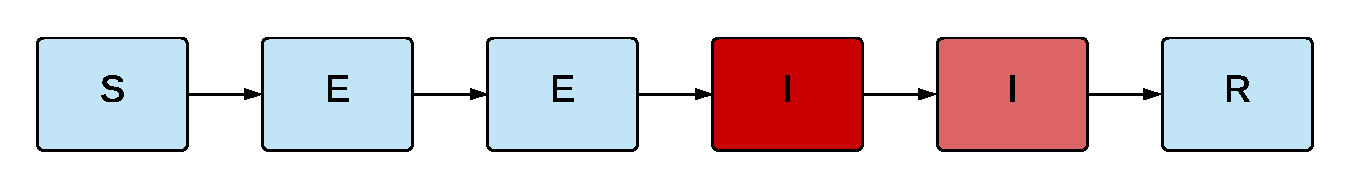
\includegraphics[width=\textwidth]{../../tex_descriptions/models/sm_sir/sm_sir_seir.pdf}
    \caption{Unstratified compartmental model structure. S = susceptible, E = exposed, I = active, R = recovered/removed. Depth of pink/red shading indicates the infectiousness of the compartment.}
    \label{fig:seeiir}
\end{figure}

\section{Model stratification}
\subsection{Model stratification}
% Note that this will vary for every application, so will need to be edited - not sure of how best to manage this:
All compartments of the base compartmental structure were stratified by age, location and organ status:\linebreak
Age
\begin{itemize}
    \item Zero to 14 years
    \item 15 to 24 years
    \item 25 to 49 years
    \item 50 to 69 years
    \item 70 years and above
\end{itemize}
Location
\begin{itemize}
    \item South Tarawa
    \item Other location
\end{itemize}
Organ status
\begin{itemize}
    \item Pulmonary smear-posivtive
    \item Pulmonary smear-negative
    \item Extrapulmonary
\end{itemize}

\section{Infectious seed}
The infectious seed value is assigned to the early infectious compartment.
This value is subtracted from the total modelled population and assigned to the susceptible compartment, while all other compartments are assigned a starting value of zero.
This process is undertaken before age stratification is applied,
with the stratification process then splitting these values proportionately according to the starting age distribution of the population.

\section{Case detection and isolation} \label{cdr}

\subsection{Determining the proportion of cases detected}
We calculate a time-varying case detection rate, being the proportion of all symptomatic cases (the second and third clinical strata) that are detected (the third clinical stratum only).
This proportion is informed by the number of tests performed using the following formula:

\[CDR(time)=1-(1-floor)\times e^{-shape \times tests(time)}\]

$time$ is the calendar date and $tests(time)$ is the number of tests per capita done on that date. To determine the value of the shape parameter, we solve this equation based on the assumption that a certain daily testing rate $tests(t)$ is associated with a certain $CDR(t)$.
$floor$ is the minimum case detection rate possible, which would theoretically occur when zero tests are conducted.
Solving for $shape$ yields:

\[shape = \frac{-log(\frac{1 - CDR(t)}{1 - floor})}{tests(t)}\]

That is, if it is assumed that a certain daily per capita testing rate is associated with a certain proportion of symptomatic cases detected, we can determine $shape$.
As this relationship is not well understood and unlikely to be consistent across all settings, we vary the $CDR$ that is associated with a certain per capita testing rate during calibration.
This approach allows us to both vary the $CDR(\cdot)$ relationship through calibration,
while also varying the specific $CDR(time)$ to reflect historical changes in testing capacity with time.

\subsection{Isolation of detected cases}
As described in the clinical stratification section above, as infected persons progress from the early to the late stage of active COVID-19, infectiousness is reduced for those detected to reflect case isolation.

\section{Parameters}
\subsection{Age-specific parameters}
Age-structured parameters are presented in Table \ref{tab:age_params}.

\begin{table}
    \begin{threeparttable}
    \begin{tabularx}{\textwidth}{| X | X | X | X | X |}
        \hline
        \textbf{Age group} (years) & \textbf{Clinical fraction} \tnote{a} & 
        \textbf{Relative susceptibility to infection} & \textbf{Case fatality rate} & 
        \textbf{Proportion of symptomatic patients hospitalised} \\
        \hline
        0 to 9   & 0.533 & 0.36 & $5\times10^{-5}$   & 0.011 \\
        \hline
        10 to 19 & 0.533 & 0.36 & $1\times10^{-5}$   & 0.0038 \\
        \hline
        20 to 29 & 0.679 & 1    & $2\times10^{-5}$   & 0.006 \\
        \hline
        30 to 39 & 0.679 & 1    & $5\times10^{-5}$   & 0.0066 \\
        \hline
        40 to 49 & 0.679 & 1    & $1\times10^{-4}$   & 0.0059 \\
        \hline
        50 to 59 & 0.679 & 1    & $5\times10^{-4}$   & 0.0077 \\
        \hline
        60 to 69 & 0.803 & 1    & $2\times10^{-3}$   & 0.0139 \\
        \hline
        70 to 79 & 0.803 & 1.41 & $8.3\times10^{-3}$ \tnote{b} & 0.0357 \tnote{b} \\
        \hline
        80 and above & 0.803 & 1.41 & $5.12\times10^{-2}$ \tnote{b} & 0.111 \tnote{b} \\
        \hline
        Justification and source & 
        Table 1 of systematic review and meta-analysis with appropriate accounting for testing during the pre-symptomatic period\cite{sah-2021}. & 
        Conversion of odds ratios presented in Table S15 of Zhang et al. 2020 to relative risks using data presented in Table S14 of the same study \cite{zhang-2020-a}. &
        Table S2 from Supplemental Materials to Nyberg et al. for ``Hospital admission up to 14 days after positive test''. &  % FIXME: Reference corrupted
        Table S2 from Supplemental Materials to Nyberg et al. for ``Death within 28 days after positive test''. \\  % FIXME: Reference corrupted
        \hline
	\end{tabularx}
	\caption{\textbf{Values used to estimate age-specific parameters.}
    Note that these base parameter values are then adjusted for immunity considerations.}
	\label{tab:age_params}
    \begin{tablenotes}
        \item[a] Proportion of incident episodes developing symptoms.
        \item[b] Modelled age groups are five year brackets to 75 and above.
        These values are used to calculated weighted value for the modelled 75 and above age bracket.
        The value for the 75 and above age group is calculated as the weighted average of the parameters for the 75 to 79 and the 80 and above age groups.
        The weights applied to each of these two groups is the size of the population in the country of application in each of these brackets.
    \end{tablenotes}
    \end{threeparttable}
\end{table}


\newpage
\printbibliography

\end{document}
